\chapter{Functional Methods in Quantum Field Theory}\label{chap:QFT}
This chapter introduces a treatment of quantum field theory using functional methods. The main goal is to get familiar with the physical concepts and the notation used throughout this work and to derive the flow equation for the average effective action, introduced by Christof Wetterich in 1993 \cite{Wetterich1992}. 
For the derivation of the flow equation we are following \cite{FloerchingerWetterichQFT, PawlowskiNPgaugeLecture}.

\section{Generating Functionals and Correlation Functions}
We consider a theory setting of $N$ real scalar fields $\varphi_a(x), a \in \{1,\dots,N\}$ in $d$-dimensional Euclidean space. The corresponding partition sum in presence of sources $J_a(x)$ reads
\begin{align}
	Z[J] = \frac{1}{\mathcal{N}} \int \D\varphi \operatorname{e}^{-\S + J\cdot\varphi}.
	\label{eqn:partition}
\end{align}
The action $\mathcal{S}$ is specified together with an ultraviolet cutoff scale $\Lambda$, later being the momentum scale where we initialize the flow equations and some normalization factor $\mathcal{N}$.

In this notation, the scalar product sums over field components and integrates over all space,
\begin{align}
	J\cdot\varphi = \int_x J_a(x) \ \varphi_a(x) = \int_p \tilde{J}_a(p) \ \tilde{\varphi}_a(p),
\end{align}
with
\begin{align}
\int_x = \int_{\mathbb{R}^d} \dd^d x \qquad \text{and} \qquad \int_p = \int_{\mathbb{R}^d} \frac{\dd^d p}{(2\pi)^d}.	
\end{align}

The partition sum $Z[J]$ is called a \textit{generating functional}. It directly allows us to compute field expectation values
\begin{align}
	\phi := \cf{\varphi} = \eval{\frac{1}{Z}\frac{\delta Z}{\delta J}}_{J=0} = \int \D\varphi \ \varphi \ \operatorname{e}^{-\S + J\cdot\varphi}
\end{align}
and higher order correlation functions
\begin{align}
\cf{\varphi_1 \cdots \varphi_n} := \cf{\varphi^n} = \frac{1}{Z}\eval{\frac{\delta^n Z}{\delta^n J}}_{J=0} = \int \D\varphi \ \overbrace{\varphi_1 \cdots \varphi_n}^{:= \ \varphi^n} \ \operatorname{e}^{-\S + J\cdot\varphi}
\end{align}
via functional differentiation.. This means, we are basically able to compute all contributing Feynman diagrams for our theory setting, if we have knowledge of its corresponding (grand) canonical partition sum. \\
 For a more efficient description of the theory in terms of only the \textit{connected} correlation functions, we define the Schwinger functional $W[J]$ as the logarithm of $Z[J]$,  
\begin{align}
W[J] = \ln Z[J].
\label{eqn:Schwinger}
\end{align}
It is the generating functional for the connected correlation functions. The normalization factor $\mathcal{N}$, introduced in (\ref{eqn:partition}) enters here as an additive constant, which drops out for all higher order correlation functions, except for the zero-point function. This term is connected to the thermodynamic quantities of our system and becomes important, when external parameters such as temperature, volume or the chemical potential are varied. For the case of quantum gravity, it is linked to the cosmological constant $\Lambda$. Nevertheless, in general we are only interested in correlation functions with $n\geq 1$ and therefore we drop this term.\\
Consider for example the connected two-point function $G_{ab}(x,y) = G_{\alpha\beta}$\footnote{To save on notation, we introduce collective indices $\alpha = (x,a)$ respectively $(q,a)$ in momentum space.}, known as the propagator, correlating the field $\varphi_a$ at spacetime point $x$ with the field $\varphi_b$ at $y$,
\begin{align}
	G_{\alpha\beta} &= \frac{\delta^2W[J]}{\delta J_{\alpha}\delta J_{\beta}} = \frac{\delta}{\delta J_{\alpha}}\left(\frac{1}{Z}\frac{\delta Z}{\delta J_{\beta}}\right) \nonumber \\[10pt]
				&= \frac{1}{Z}\left(\frac{\delta^2Z}{\delta J_{\alpha}\delta J_{\beta}}\right) - \frac{1}{Z^2}\left(\frac{\delta Z}{\delta J_{\alpha}}\right)\left(\frac{\delta Z}{\delta J_{\beta}}\right)\\[10pt]
				&= \cf{\varphi_{\alpha}\varphi_{\beta}} - \phi_{\alpha}\phi_{\beta} = \cf{\varphi_{\alpha}\varphi_{\beta}}_{\text{c}}.	\nonumber	
\end{align}
The propagator is the key object in functional approaches to quantum field theory. It depends on the chosen background via $J$. \\
It is still possible to make our computations even more efficient, because $W[J]$ still contains some redundant information. Connected correlation functions can be separated into so-called one-particle irreducible (1PI) and one-particle reducible ones. The 1PI correlation functions are those, whose corresponding Feynman diagrams can \textit{not} be separated into two disconnected ones by cutting a single internal line. As an example, contributing 1PI and reducible diagrams to the connected four-point function for Yukawa theory, are depicted in figure (\ref{fig:1PI_Yukawa}). 
\begin{figure}[t]
\centering
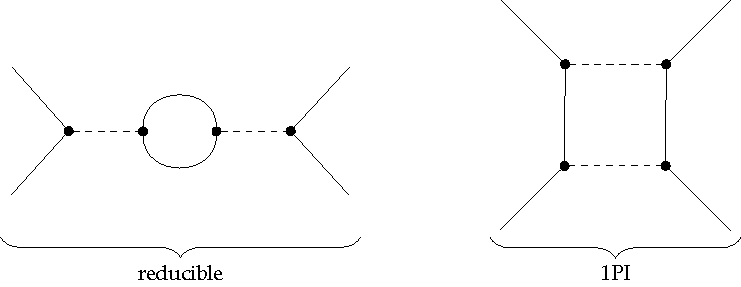
\includegraphics[width=0.8\textwidth]{figs/TikZ/1PI_Yukawa}
\caption{Contributing one-particle reducible and 1PI diagrams to the four-point-function in Yukawa theory.}	
\label{fig:1PI_Yukawa}
\end{figure}

The generating functional for the  1PI correlation functions, the \textit{effective action} $\Gamma$, is obtained from the Schwinger functional via a Legendre transform, 
\begin{align}
	\Gamma[\phi]=\sup _{J}\left\{\int_{x} J(x) \phi(x)-W[J]\right\}=\int_{x} J_{\mathrm{sup}}(x) \phi(x)-W\left[J_{\mathrm{sup}}\right],
\end{align}
where $J_{\mathrm{sup}}$ has to be understood as a field-dependent current $J_{\mathrm{sup}}[\phi]$. In the following, we will drop the subscript, its meaning is implicitly understood.  From a physical point of view, the effective action $\Gamma$ is the quantum analogue of the classical action $\mathcal{S}$. The performed Legendre transform leads us to a mean field description of our theory with $\phi = \cf{\varphi}$ on a given background, as introduced before. The symmetries of the classical action are in general still present in the effective action.\\
In terms of the effective action, correlation functions are again obtained by performing functional derivatives, but now w.\,r.\,t. the mean field $\phi$,
\begin{align}
	\Gamma^{(n)}\left(x_{1}, \ldots, x_{n}\right)=\frac{\delta^{n} \Gamma}{\delta \phi\left(x_{1}\right) \cdots \delta \phi\left(x_{n}\right)}.
\end{align}
For the transition from connected to 1PI correlation functions we have to convert $J$- derivatives into $\phi$-derivatives, i.\,e.
\begin{align}
	\frac{\delta}{\delta J(x)}=\int_{y} \frac{\delta \phi(y)}{\delta J(x)} \frac{\delta}{\delta \phi(y)}=\int_{y} G(x, y) \frac{\delta}{\delta\phi(y)},
\end{align}
where we used, that $\sfrac{\delta\phi}{\delta J} = \sfrac{\delta W^{(1)}}{\delta J} = G.$ Evaluating the product of the two two-point functions obtained from $W$ and $\Gamma$ respectively, gives us another important result:
\begin{align}
 \int_{y} \frac{\delta^{2} W}{\delta J\left(x_{1}\right) \delta J(y)} \frac{\delta^{2} \Gamma}{\delta \phi(y) \delta\phi\left(x_{2}\right)} &=\int_{y} \frac{\delta}{\delta J\left(x_{1}\right)}\left[\frac{\delta W}{\delta J(y)}\right] \frac{\delta}{\delta \phi(y)}\left[\frac{\delta \Gamma}{\delta \phi\left(x_{2}\right)}\right] \nonumber\\[10pt]
	&=\int_{y} \frac{\delta \phi(y)}{\delta J\left(x_{1}\right)} \frac{\delta}{\delta \phi(y)} J\left(x_{2}\right) \\[10pt] 
	&=\delta_{\mathrm{D}}\left(x_{1}-x_{2}\right).\nonumber
\end{align} 
The full propagator $G$ is the inverse of the 1PI two-point function:
\begin{align}
	W^{(2)}(x_1,x_2) = G(x_1,x_2) = \frac{1}{\Gamma^{(2)}}(x_1,x_2).
\end{align}
 In the next section, we want to use these concepts to introduce the functional renormalization group (FRG)... 
\section{Functional Renormalization Group}
The functional renormalization group is a mathematical tool, allowing us to investigate the dynamics of physical systems on different scales, i.\,e. energy or momentum scales. This idea is based on a continuous version of Kadanoffs block spin model on the lattice and was developed by Kenneth G. Wilson in 1971. It aims at solving the theory by integrating successively momentum shell by momentum shell, being the reason why the path integral approach to quantum field theory, as introduced before, provides a suitable framework. The main advantage of the FRG approach is, that no regularization or renormalization procedure has to be applied. The latter one is already implemented systematically, which secures the self-consistency of the approach.

As a first step towards a FRG equation we need to introduce an infrared cutoff scale $k$ in our theory, below which the modes are not integrated out. A common way to introduce such a scale is by  adding a scale-dependent cutoff term $\Delta\mathcal{S}_k$ in the definition of the partition sum (\ref{eqn:partition}) and therefore automatically also in the definition of the Schwinger functional (\ref{eqn:Schwinger})
\begin{align}
W_{k}[J]=\ln Z_{k}[J]=\ln \int \mathcal{D} \varphi  \operatorname{e}^{-\mathcal{S}[\varphi]+J \cdot \varphi-\Delta \mathcal{S}_{k}[\varphi]}.
\label{eqn:Wk}
\end{align}
The physical scale $k$ we introduced here is known as \textit{renormalization scale} and has units of inverse length, meaning large $k$ correspond to small distances and vice versa. The cutoff term $\Delta\mathcal{S}_k$ is a quadratic functional depending on the field $\varphi$,
\begin{align}
	\Delta \mathcal{S}_{k}[\varphi]=\frac{1}{2} \varphi \cdot R_{k} \cdot \varphi=\frac{1}{2} \int_{x, y} \varphi_{\alpha} \ R_{k, \alpha\beta} \ \varphi_{\beta}.
\end{align}
The function $R_k$ is called regulator. It plays an important role for this formulation of quantum field theory. The regulator is chosen such that only the propagation for momentum modes with $p^2 \lesssim k^2$ is suppressed. The most important physical limits are summarized in the following:
\begin{align}
	R_{k}(p^2) \rightarrow\left\{\begin{array}{ll}{k^{2}} & {\text { for } p \rightarrow 0} \\ {0} & {\text { for } p \rightarrow \infty} \\ {0} & {\text { for } k \rightarrow 0} \\ {\infty} & {\text { for } k \rightarrow \Lambda}\end{array}\right.
\end{align}
We will come back to these limits after deriving the FRG equation, to get a deeper insight into the physical interpretation of the regulator.
A convenient choice of the regulator is given by
\begin{align}
	R_k(p^2) = p^2 \cdot r_k(y),
\end{align}
with $ y := \frac{p^2}{k^2}$, and a dimensionless regulator shape function $r_k$, only depending on the dimensionless momentum ratio $\sfrac{p^2}{k^2}$. There is a plethora of different types of shape functions. For the computations performed in this work, we restrict ourselves to a class of rather simple, so-called Litim-type regulators with shape functions
\begin{align}
r_k(y) = \left(\frac{1}{y} - 1\right)\theta(1-y),	
\end{align}
where $\theta$ is the Heaviside step function. This class of (sharp) regulators is a good choice for finding analytic FRG equations in simple approximations. For numerical approaches, exponential regulators, which are in general more complicated, are well suited.
In this setting, (\ref{eqn:Wk}) provides a good starting point for solving the theory by successively lowering the cutoff scale $k$ infinitesimally and integrating out all momentum modes $\varphi_{p\approx k}$. \\
This procedure can be formalized by taking a scale derivative of our scale-dependent functional (\ref{eqn:Wk})
\begin{align}
k\partial_k W_k[J]= -\cf{k\partial_k\Delta\mathcal{S}_k[\varphi]}.	
\end{align}
At this point it is quite convenient to introduce derivatives w.\,r.\,t. the \textit{RG time} $t$ as
\begin{align}
	\partial_t = \frac{\partial}{\partial\ln(k/\Lambda)} = \frac{k}{\Lambda}\frac{\partial}{\partial(k/\Lambda)} = k \partial_k,
\end{align}
where $\Lambda$ is a fixed reference scale. Usually one chooses the ultraviolet cutoff scale, where the flow is initialized.

%TODO: Finish derivation!

With the definition of the propagator, we finally arrive at the FRG equation, also called Wetterich equation or flow equation for the effective action:
\begin{subequations}
\begin{align}
	\partial_t\Gammak[\phi] &= \frac{1}{2}\tr{\left(\Gammak^{(2)}[\phi] + R_k\right)^{-1} \partial_t R_k} \nonumber \\ \phantom{.}  \\
							&= \frac{1}{2}\int_p \left(\Gammak^{(2)}[\phi] + R_k\right)^{-1}(p, -p) \ \partial_t R_k(p^2). \nonumber
\label{eqn:Wetterich}							
\end{align}
It has a rather simple diagrammic representation as one-loop equation:

\begin{figure}[H]
\centering
\begin{gather}
\begin{aligned}
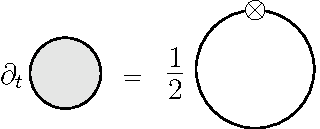
\includegraphics[scale=1.1]{figs/TikZ/wetterich_equation}
\end{aligned}
\end{gather}
\end{figure}
\end{subequations}
 where $\partial_{t} R_{k, ij}(p, q)=\partial_{t} R_{k}(p^2)(2 \pi)^{d} \  \delta_{i j} \ \delta_{\mathrm{D}}(p-q)$ and therefore the trace on the r.\,h.\,s. effectively sums over just one index $i$ and integrates over one loop momentum $p$.

%TODO: Back to regulator properties...

\begin{figure}[t]
\centering
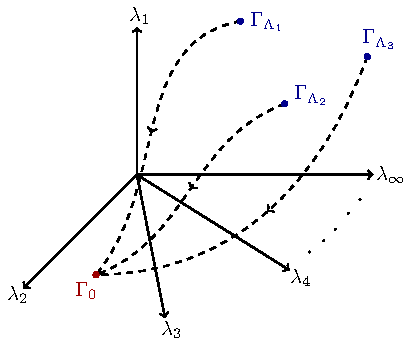
\includegraphics{figs/TikZ/regulator_dependence}
\caption{Flow of $\Gamma_k$ through infinite-dimensional theory space for different regulators.}	
\end{figure}



\section{Systematic expansion schemes}
%Derivative expansion, vertex expansion and other stuff �